
% preamble to the OGTC logic report compiler
% This piece of code consists of initializing
% the code and declaring colors, packages and 
% command changes such as the section headings
% the document is aimed to be as consise as possible
% please keep this in mind when expanding or 
% editing the code


\documentclass{article}
%% declare used packages
\usepackage{lipsum}
\usepackage[english]{babel}
\usepackage[defaultfam,tabular,lining]{montserrat} 
\usepackage[a4paper, left=1.5cm, right=1.5cm, bindingoffset=0cm]{geometry}
\usepackage{multicol} % multiple columns
\usepackage{fancyhdr} % header and footer
\usepackage{titlesec} % remove spacing around section titles, underline section titles
\usepackage{tikz}     % header and footer
\usepackage{currency} % euro sign
\usepackage{caption}
%\usepackage{amsmath}
%% Declares the logic colors
% primary colors
\definecolor{primblue}{RGB}{0,79,159}
\definecolor{primwhite}{RGB}{255,255,253}

% secondary colors
\definecolor{secdarkblue}{RGB}{35,57,101}
\definecolor{seclightblue}{RGB}{0,139,210}
\definecolor{secyellow}{RGB}{253,194,0}
\definecolor{secgray}{RGB}{207,208,208}

% define euro as currency
\DefineCurrency{EUR}{name={euro},pre=true,plural={euros},symbol={\euro},iso={EUR},kind=symbol,base=2}

% page style
\usetikzlibrary{calc}
\renewcommand{\headrulewidth}{0pt}

\pagestyle{fancy}
\fancyhf{}
\fancyhead[C]{%
\begin{tikzpicture}[overlay, remember picture]%
    \fill[primblue] (current page.north west) rectangle ($(current page.north east)+(0,-1in)$);
    \node[anchor=north west, text=white, font=\LARGE\scshape, minimum size=1in, inner xsep=15mm] at (current page.north west) {Microgrid sizing by OGTC's LOGiC sizing tool};
    \node[anchor=north east, minimum size=1in, inner xsep=5mm] at (current page.north east) {
\includegraphics[scale=.1]{logo.png}};
      %node[minimum width=\x2-\x1, minimum height=2cm, draw, rectangle, fill=blue!20, anchor=north west, align=left, text width=\x2-\x1] at ($(current page.north west)$) {\Large\bfseries \quad #1};
\end{tikzpicture}
}
\fancyfoot[C]{
    \begin{tikzpicture}[overlay, remember picture]%
    \fill[primblue] (current page.south west) rectangle ($(current page.south east)+(0,.5in)$);
    \node[anchor=south west, text=white, font=\Large, minimum size=.5in] at (current page.south west) {\thepage};
    \node[anchor=south, text=white, font=\large, minimum size=.5in] at (current page.south) {\leftmark};
    \node[anchor=south east, text=white, font=\large, minimum size=.5in, inner xsep=5mm] at (current page.south east) {\today};
\end{tikzpicture}
}
\fancyfoot[CO]{
    \begin{tikzpicture}[overlay, remember picture]%
    \fill[primblue] (current page.south west) rectangle ($(current page.south east)+(0,.5in)$);
    \node[anchor=south west, text=white, font=\large, minimum size=.5in, inner xsep=5mm] at (current page.south west) {www.offgridtestcenter.nl};
    \node[anchor=south, text=white, font=\large, minimum size=.5in] at (current page.south) {\leftmark};
    \node[anchor=south east, text=white, font=\large, minimum size=.5in] at (current page.south east) {info@offgridtestcenter.nl};
\end{tikzpicture}
}
%\setlength{\headheight}{12pt}
\setlength\columnsep{10mm}
\renewcommand{\arraystretch}{1.2}
\titlespacing*{\section}{0pt}{2.5mm}{0mm} % make spacing smaller
\titleformat{\section}
    {\normalfont\Large\bfseries}{\thesection}{1em}{}[\color{primblue}\titlerule\vspace*{4pt}]
    
\newenvironment{Figure}
  {\par\medskip\noindent\minipage{\linewidth}}
  {\endminipage\par\medskip}

\begin{document}

\begin{multicols*}{2}

This document shortly reports the results of the use of the LOGiC sizing tool. This introduction describes the input values used to perform the calculations.The system is assumed to be located at or close to dumadr.

\section*{Microgrids}

In order to make this report comprehendable to the user the general properties of a microgrid are shortly discussed.\\ A microgrid is a local energy system that is capable of generating, storing and delivering energy locally. Microgrids can be both connected to the main grid (grid-connected microgrids) as well as being completely isolated (off-grid microgrids). The microgrid considered in this assessment is a off-grid microgrid. This means that the microgrid has to generate all electrical energy consumed in the grid locally and that no extra energy can be bought from external parties. Shortages are fulfilled by using a back-up diesel generator. There multpile possible reasons to apply a microgrid: \begin{itemize}

 \item No grid is available (remote location) 

\item There is a grid availble, but is is not reliable (enough)  

\item The wish to generate the own energy locally as a stakeholder or a community 

\end{itemize}

In all cases renewable sources are often considered as a possible source of energy for the microgrid, either from an economic or a sustainable driver. In the case of this microgrid the following sources are considered: wind power, solar power and a back-up generator combined with a storage facility.

\section*{System sizing}

The calculation described above has resulted in the following system:

\begin{center}

\begin{tabular}{|l|r|}

\hline Component&Capacity\\ \hline 

Installed solar power&0.0\\ 

Installed wind power&21.26914\\ 

Installed storage capacity&8.27409\\ 

Power of storage facility&4.13705\\ 

\hline

\end{tabular}

\label{tab:systemlayout}

\end{center}

\captionof{table}{Sizing of the main components of the system}

\vspace{2.5mm}

The system defined by the parameters above realises a levelised cost of electricity of \texteuro 0.43 per kWh. the system does this at a renewable energy share of 0.01 \%. 

\section*{System economics}

In order to assess the economics of the system the following economic parameters have been assumed: 

\begin{center}

\begin{tabular}{|l|r|c|}

\hline Parameter&Value&Units\\ \hline 

\hline

\end{tabular}

\label{tab:econinputtable}

\end{center}

\captionof{table}{Economic input variables}

\vspace{2.5mm}

Based on these the investment costs of the main components of the system are estimated as:

\begin{center}

\begin{tabular}{|l|r|c|}

\hline Component&Investment cost\\ \hline 

Solar modules&0.0\\ 

Wind turbines&53172.8595\\ 

Storage facility&2710.1694\\ 

\hline

\end{tabular}

\label{tab:investtable}

\end{center}

\captionof{table}{Investment cost of the system}

\vspace{2.5mm}

The operational expenditure is estimated as:

\begin{center}

\begin{tabular}{|l|r|c|}

\hline Component&Annual pu OPEX&Units\\ \hline 

Solar panels&25.0&kWp\\ 

Wind turbines&0.0&kW\\ 

Storage capacity&6.75&kWh\\ 

Storage power&0.0&kW\\ 

\hline

\end{tabular}

\label{tab:opextable}

\end{center}

\captionof{table}{Operational expenditure of the main components of the system}

\vspace{2.5mm}



\section*{Societal environment}

Apart from the quantitative factors tht determine the sizing of the system in the technical sense, there are also societal, quantitative factors that should be taken into account when making investment decisions regarding the installation of an (off-grid) microgrid. This section gives some important societal factors.

\subsection{first}

first societal factor

\section*{Conclusion}

body text

\newpage 

\appendix

\section*{Used input data and method}

The timeseries used in and resulting from the calculations are listed on this page.

\begin{center}/r/n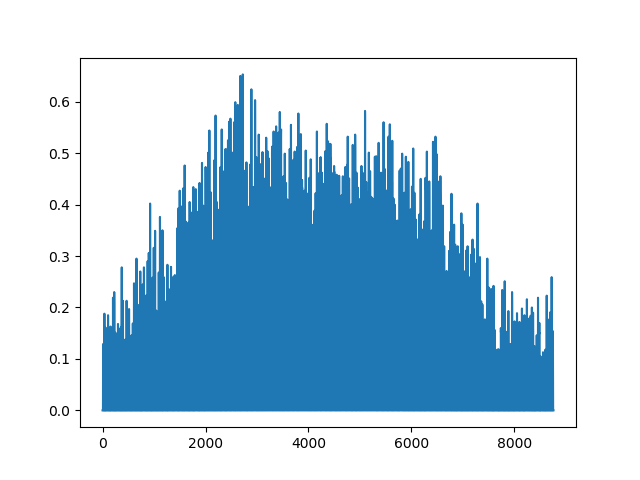
\includegraphics[width=\linewidth]{per_unit_pv_generation.png}/r/n\end{center}/r/n\captionof{figure}{Time series of the solar energy production in kW per kWp of installed solar power}/r/n



\begin{center}/r/n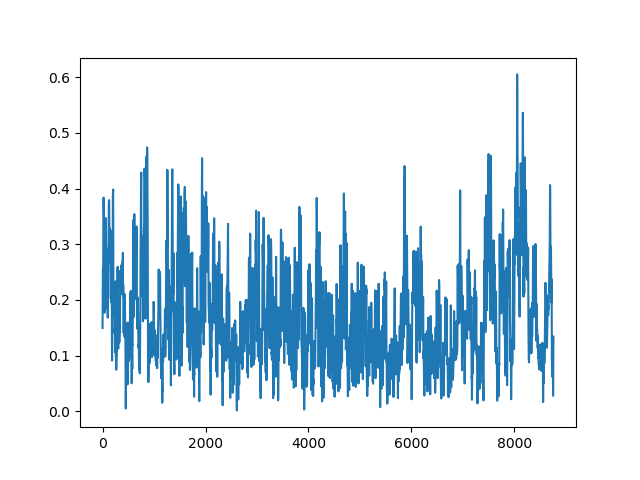
\includegraphics[width=\linewidth]{per_unit_wind_generation.png}/r/n\end{center}/r/n\captionof{figure}{Time series of the wind energy production in kW per kW of installed wind power}/r/n





\end{multicols*}

\end{document}